\section{Content Impact}

One aim of this research is to analyze the impact posting new content has on super-users' followers counts.

To this end, all videos posted by a super-user were downloaded over the span of five months. For each video, all new followers within five days from the upload date were registered.

\begin{lstlisting}[language=json]
{
    "data": {
        "cursor": 1717588518,
        "has_more": true,
        "user_followers": [
            {
                "username": "rev6luv",
                "display_name": "t."
            },
            {
                "display_name": "Caden M. Flanagan",
                "username": "therealcadenflanagan"
            },
            ...
    }
} 
\end{lstlisting}

There is a potential bias in this approach, as new followers can be gained independently of posted content. However, in the current social network landscape, content either goes viral almost immediately or not at all. For this reason, this approach has been considered valid.

The query included in the body of the request contains only the username, without filtering other parameters (such as hashtag, or region). This decision has been made since a super-user, while eclectic in the topics discussed, still belongs to a specific political orientation.

\begin{lstlisting}[language=json, label={lst:query}]
{
    "and": [
        {
            "operation": "IN",
            "field_name": "username",
            "field_values": [
                "$influencer" 
            ]
        }
    ]
}
\end{lstlisting}

In this analysis, only the most influential super-users have been considered (those with more followers and higher engagement values):

\begin{figure}[H]
    \centering
    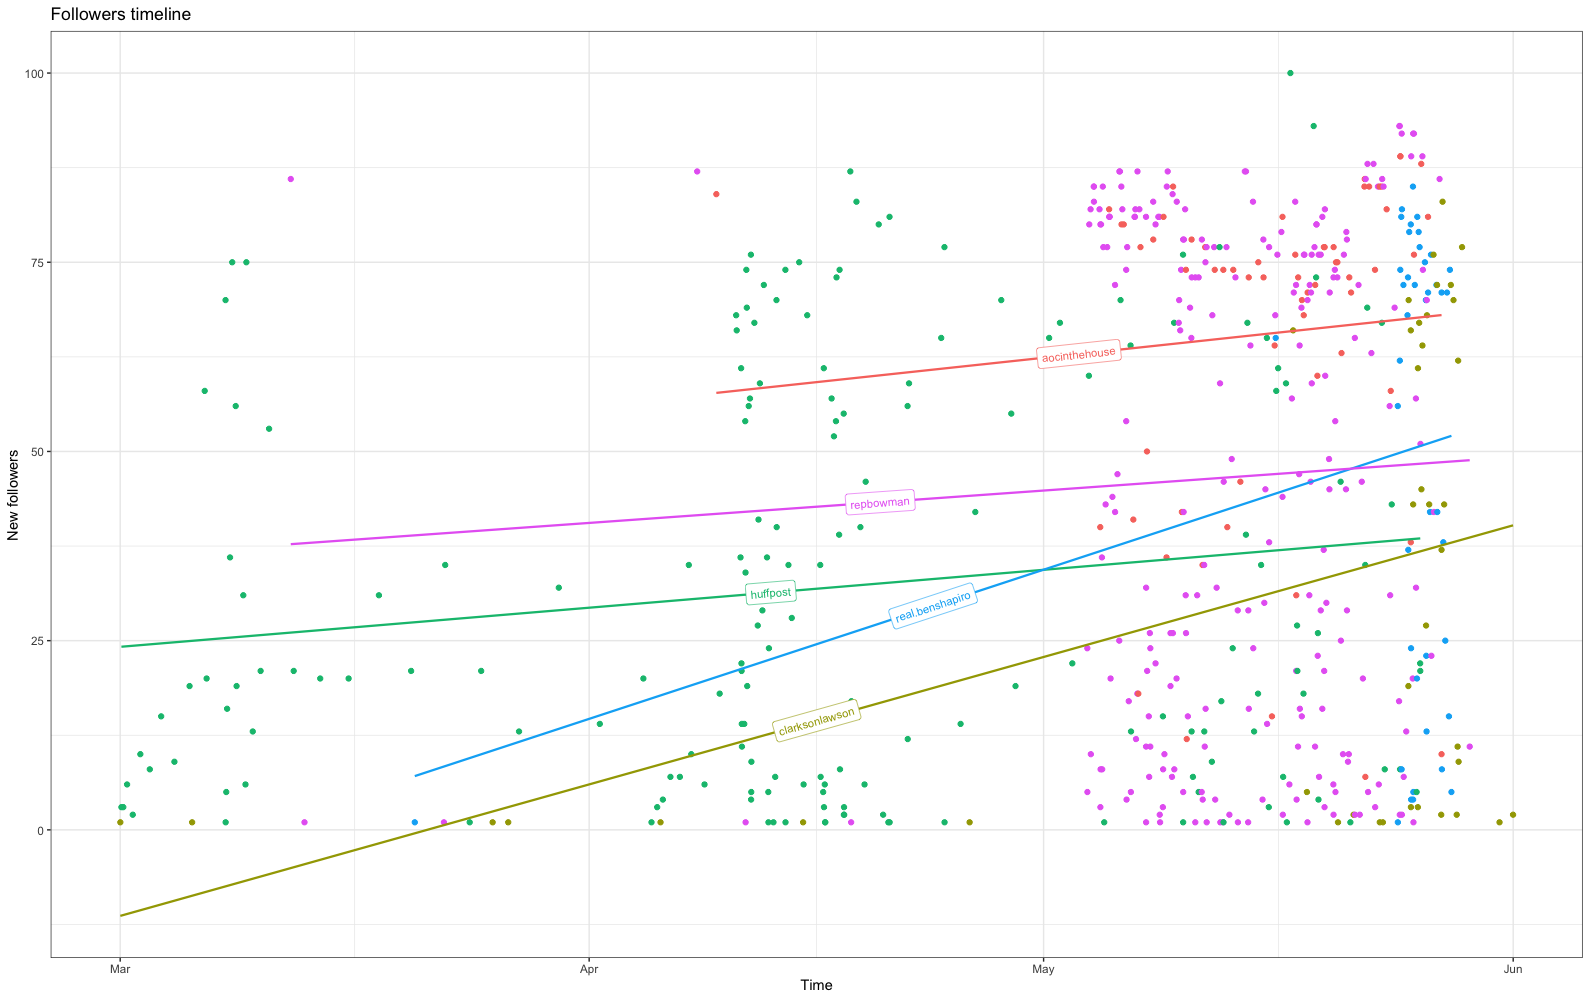
\includegraphics[width = .48\textwidth]{images/Final_Followers_Timeline.png}
    \caption*{As can be seen, the total number of followers increases steadily over time for almost all super-users.}
\end{figure}

A more specific analysis has been done on two super-users of particular interest: \textit{@aocinthehouse} and \textit{@real.benshapiro}:

\begin{figure}[H]
    \centering
    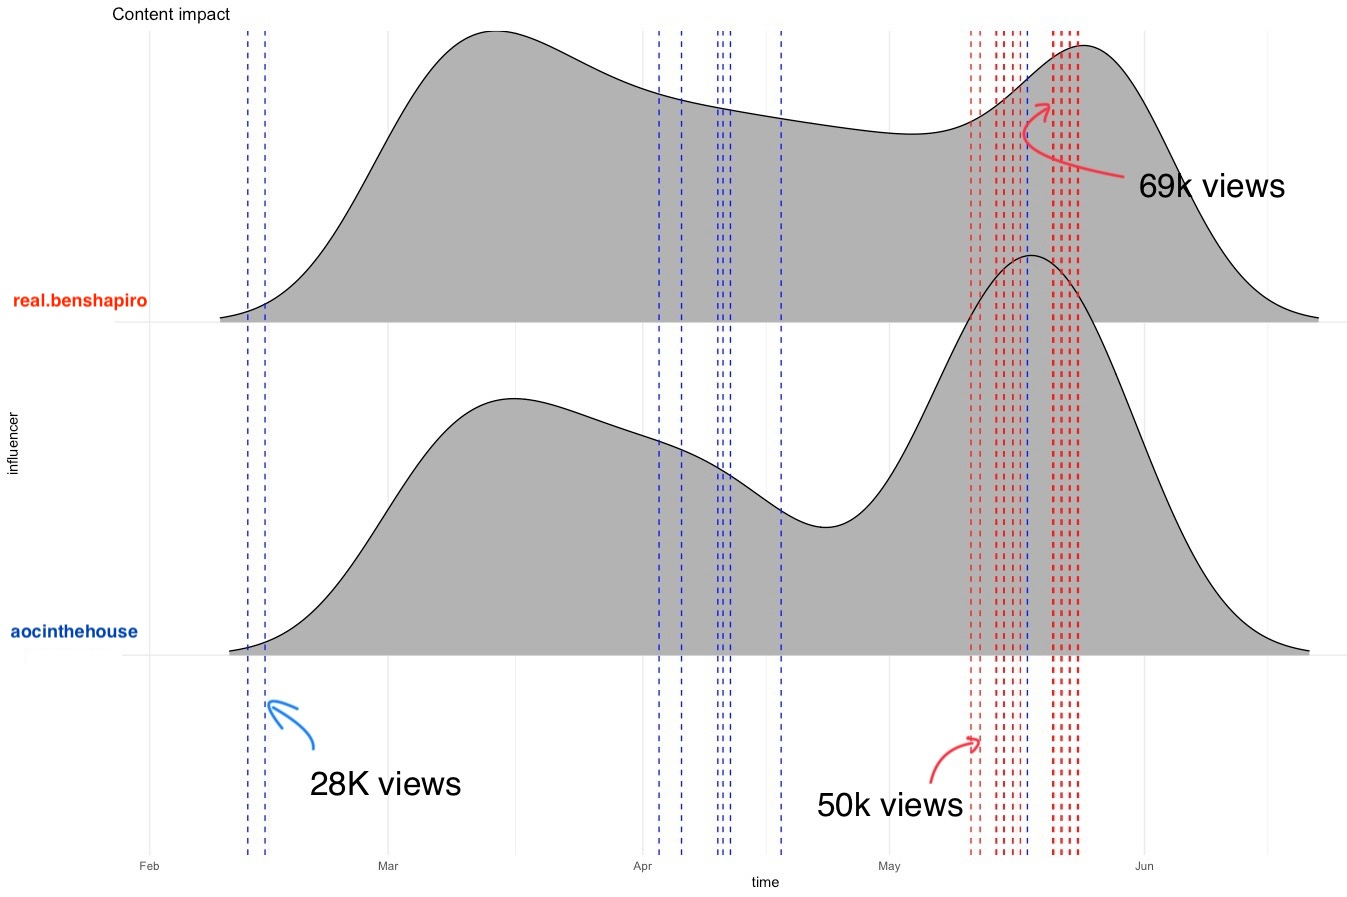
\includegraphics[width = .48\textwidth]{images/Final_ContentImpact_Custom.jpg}
    \caption*{This analysis consisted of the average trend of new followers, creating a detailed curve enriched with timestamps of new post creations.}
\end{figure}

In the graph shown above, there is a noticeable increase in new followers for \textit{@aocinthehouse} after the content posted on 15 February was viewed 28,000 times.

The aforementioned bias is evident in the increase in \textit{@real.benshapiro}'s follower count in mid-March despite not being active on TikTok. It can be inferred that influence on followers' count extends beyond TikTok, supported by the release of a YouTube video on 9 March 2024, which received nearly 300,000 views.